\documentclass{standalone}
\usepackage{tikz}
\usetikzlibrary{patterns, positioning}


\begin{document}
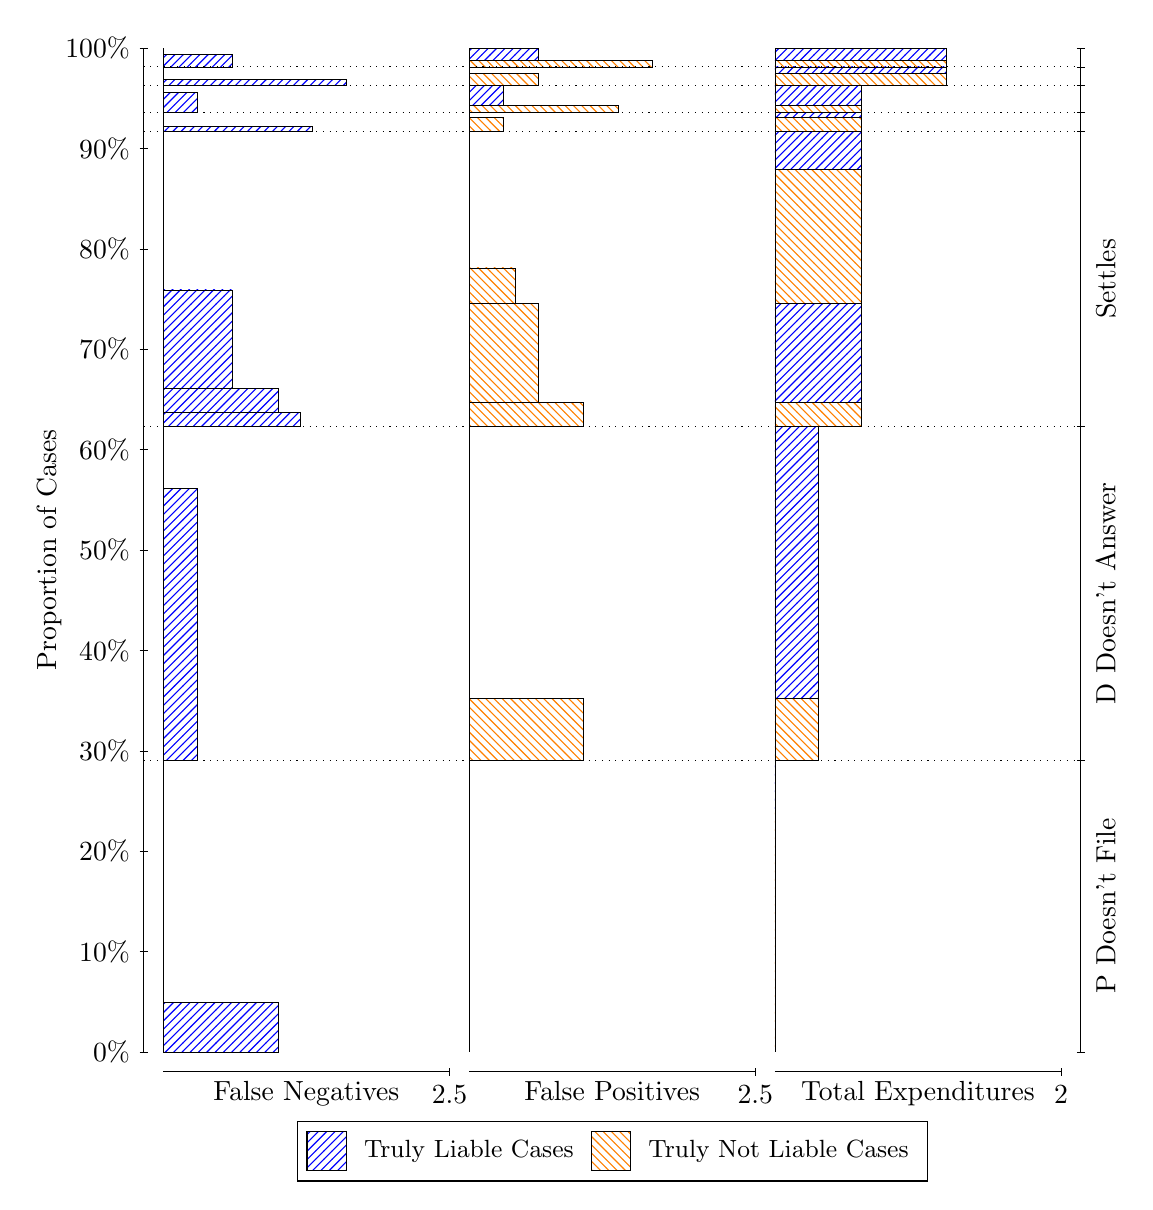
\begin{tikzpicture}
\draw[black, very thin] (1.5,1.75) -- (1.5,14.5);
\node[rotate=90, text=black, anchor=center] at (0.3, 8.125) {Proportion of Cases};
\draw[black, very thin] (1.45,1.75) -- (1.55,1.75);
\node[text=black, anchor=east] at (1.45, 1.75) {0\%};
\draw[black, very thin] (1.45,3.025) -- (1.55,3.025);
\node[text=black, anchor=east] at (1.45, 3.025) {10\%};
\draw[black, very thin] (1.45,4.3) -- (1.55,4.3);
\node[text=black, anchor=east] at (1.45, 4.3) {20\%};
\draw[black, very thin] (1.45,5.575) -- (1.55,5.575);
\node[text=black, anchor=east] at (1.45, 5.575) {30\%};
\draw[black, very thin] (1.45,6.85) -- (1.55,6.85);
\node[text=black, anchor=east] at (1.45, 6.85) {40\%};
\draw[black, very thin] (1.45,8.125) -- (1.55,8.125);
\node[text=black, anchor=east] at (1.45, 8.125) {50\%};
\draw[black, very thin] (1.45,9.4) -- (1.55,9.4);
\node[text=black, anchor=east] at (1.45, 9.4) {60\%};
\draw[black, very thin] (1.45,10.675) -- (1.55,10.675);
\node[text=black, anchor=east] at (1.45, 10.675) {70\%};
\draw[black, very thin] (1.45,11.95) -- (1.55,11.95);
\node[text=black, anchor=east] at (1.45, 11.95) {80\%};
\draw[black, very thin] (1.45,13.225) -- (1.55,13.225);
\node[text=black, anchor=east] at (1.45, 13.225) {90\%};
\draw[black, very thin] (1.45,14.5) -- (1.55,14.5);
\node[text=black, anchor=east] at (1.45, 14.5) {100\%};

\draw[black, very thin] (13.4,1.75) -- (13.4,14.5);
\draw[black, very thin] (13.35,1.75) -- (13.45,1.75);
\node[anchor=west] at (13.35, 1.75) {};
\draw[black, very thin] (13.35,5.4563) -- (13.45,5.4563);
\node[anchor=west] at (13.35, 5.4563) {};
\draw[black, very thin] (13.35,9.6954) -- (13.45,9.6954);
\node[anchor=west] at (13.35, 9.6954) {};
\draw[black, very thin] (13.35,13.441) -- (13.45,13.441);
\node[anchor=west] at (13.35, 13.441) {};
\draw[black, very thin] (13.35,13.678) -- (13.45,13.678);
\node[anchor=west] at (13.35, 13.678) {};
\draw[black, very thin] (13.35,14.022) -- (13.45,14.022);
\node[anchor=west] at (13.35, 14.022) {};
\draw[black, very thin] (13.35,14.261) -- (13.45,14.261);
\node[anchor=west] at (13.35, 14.261) {};
\draw[black, very thin] (13.35,14.5) -- (13.45,14.5);
\node[anchor=west] at (13.35, 14.5) {};

\draw[black, very thin, pattern color=blue, pattern=north east lines] (1.75,1.75) rectangle (3.2033,2.3819);
\draw[black, very thin, pattern color=orange, pattern=north west lines] (1.75,2.3819) rectangle (1.75,5.4563);
\draw[black, very thin, pattern color=blue, pattern=north east lines] (1.75,5.4563) rectangle (2.186,8.911);
\draw[black, very thin, pattern color=orange, pattern=north west lines] (1.75,8.911) rectangle (1.75,9.6954);
\draw[black, very thin, pattern color=blue, pattern=north east lines] (1.75,9.6954) rectangle (3.494,9.8681);
\draw[black, very thin, pattern color=blue, pattern=north east lines] (1.75,9.8681) rectangle (3.2033,10.175);
\draw[black, very thin, pattern color=blue, pattern=north east lines] (1.75,10.175) rectangle (2.622,11.429);
\draw[black, very thin, pattern color=orange, pattern=north west lines] (1.75,11.429) rectangle (1.75,13.441);
\draw[black, very thin, pattern color=blue, pattern=north east lines] (1.75,13.441) rectangle (3.6393,13.502);
\draw[black, very thin, pattern color=orange, pattern=north west lines] (1.75,13.502) rectangle (1.75,13.678);
\draw[black, very thin, pattern color=blue, pattern=north east lines] (1.75,13.678) rectangle (2.186,13.932);
\draw[black, very thin, pattern color=orange, pattern=north west lines] (1.75,13.932) rectangle (1.75,14.022);
\draw[black, very thin, pattern color=blue, pattern=north east lines] (1.75,14.022) rectangle (4.0753,14.106);
\draw[black, very thin, pattern color=orange, pattern=north west lines] (1.75,14.106) rectangle (1.75,14.261);
\draw[black, very thin, pattern color=blue, pattern=north east lines] (1.75,14.261) rectangle (2.622,14.416);
\draw[black, very thin, pattern color=orange, pattern=north west lines] (1.75,14.416) rectangle (1.75,14.5);
\draw[black, very thin, pattern color=orange, pattern=north west lines] (5.6333,1.75) rectangle (5.6333,4.8244);
\draw[black, very thin, pattern color=blue, pattern=north east lines] (5.6333,4.8244) rectangle (5.6333,5.4563);
\draw[black, very thin, pattern color=orange, pattern=north west lines] (5.6333,5.4563) rectangle (7.0867,6.2407);
\draw[black, very thin, pattern color=blue, pattern=north east lines] (5.6333,6.2407) rectangle (5.6333,9.6954);
\draw[black, very thin, pattern color=orange, pattern=north west lines] (5.6333,9.6954) rectangle (7.0867,10.002);
\draw[black, very thin, pattern color=orange, pattern=north west lines] (5.6333,10.002) rectangle (6.5053,11.256);
\draw[black, very thin, pattern color=orange, pattern=north west lines] (5.6333,11.256) rectangle (6.2147,11.707);
\draw[black, very thin, pattern color=blue, pattern=north east lines] (5.6333,11.707) rectangle (5.6333,13.441);
\draw[black, very thin, pattern color=orange, pattern=north west lines] (5.6333,13.441) rectangle (6.0693,13.616);
\draw[black, very thin, pattern color=blue, pattern=north east lines] (5.6333,13.616) rectangle (5.6333,13.678);
\draw[black, very thin, pattern color=orange, pattern=north west lines] (5.6333,13.678) rectangle (7.5227,13.767);
\draw[black, very thin, pattern color=blue, pattern=north east lines] (5.6333,13.767) rectangle (6.0693,14.022);
\draw[black, very thin, pattern color=orange, pattern=north west lines] (5.6333,14.022) rectangle (6.5053,14.176);
\draw[black, very thin, pattern color=blue, pattern=north east lines] (5.6333,14.176) rectangle (5.6333,14.261);
\draw[black, very thin, pattern color=orange, pattern=north west lines] (5.6333,14.261) rectangle (7.9587,14.345);
\draw[black, very thin, pattern color=blue, pattern=north east lines] (5.6333,14.345) rectangle (6.5053,14.5);
\draw[black, very thin, pattern color=orange, pattern=north west lines] (9.5167,1.75) rectangle (9.5167,4.8244);
\draw[black, very thin, pattern color=blue, pattern=north east lines] (9.5167,4.8244) rectangle (9.5167,5.4563);
\draw[black, very thin, pattern color=orange, pattern=north west lines] (9.5167,5.4563) rectangle (10.062,6.2407);
\draw[black, very thin, pattern color=blue, pattern=north east lines] (9.5167,6.2407) rectangle (10.062,9.6954);
\draw[black, very thin, pattern color=orange, pattern=north west lines] (9.5167,9.6954) rectangle (10.607,10.002);
\draw[black, very thin, pattern color=blue, pattern=north east lines] (9.5167,10.002) rectangle (10.607,11.256);
\draw[black, very thin, pattern color=orange, pattern=north west lines] (9.5167,11.256) rectangle (10.607,12.961);
\draw[black, very thin, pattern color=blue, pattern=north east lines] (9.5167,12.961) rectangle (10.607,13.441);
\draw[black, very thin, pattern color=orange, pattern=north west lines] (9.5167,13.441) rectangle (10.607,13.616);
\draw[black, very thin, pattern color=blue, pattern=north east lines] (9.5167,13.616) rectangle (10.607,13.678);
\draw[black, very thin, pattern color=orange, pattern=north west lines] (9.5167,13.678) rectangle (10.607,13.767);
\draw[black, very thin, pattern color=blue, pattern=north east lines] (9.5167,13.767) rectangle (10.607,14.022);
\draw[black, very thin, pattern color=orange, pattern=north west lines] (9.5167,14.022) rectangle (11.697,14.176);
\draw[black, very thin, pattern color=blue, pattern=north east lines] (9.5167,14.176) rectangle (11.697,14.261);
\draw[black, very thin, pattern color=orange, pattern=north west lines] (9.5167,14.261) rectangle (11.697,14.345);
\draw[black, very thin, pattern color=blue, pattern=north east lines] (9.5167,14.345) rectangle (11.697,14.5);
\draw[black, dotted] (1.5,5.4563) -- (13.4,5.4563);
\draw[black, dotted] (1.5,9.6954) -- (13.4,9.6954);
\draw[black, dotted] (1.5,13.441) -- (13.4,13.441);
\draw[black, dotted] (1.5,13.678) -- (13.4,13.678);
\draw[black, dotted] (1.5,14.022) -- (13.4,14.022);
\draw[black, dotted] (1.5,14.261) -- (13.4,14.261);
\draw[black, very thin] (1.75,1.5) -- (5.3833,1.5);
\node[text=black, anchor=north] at (3.5667, 1.5) {False Negatives};
\draw[black, very thin] (5.3833,1.45) -- (5.3833,1.55);
\node[text=black, anchor=north] at (5.3833, 1.45) {2.5};

\draw[black, very thin] (5.6333,1.5) -- (9.2667,1.5);
\node[text=black, anchor=north] at (7.45, 1.5) {False Positives};
\draw[black, very thin] (9.2667,1.45) -- (9.2667,1.55);
\node[text=black, anchor=north] at (9.2667, 1.45) {2.5};

\draw[black, very thin] (9.5167,1.5) -- (13.15,1.5);
\node[text=black, anchor=north] at (11.333, 1.5) {Total Expenditures};
\draw[black, very thin] (13.15,1.45) -- (13.15,1.55);
\node[text=black, anchor=north] at (13.15, 1.45) {2};

\node[text=black, centered, rotate=90] at (13.72, 3.6031) {P Doesn't File};
\node[text=black, centered, rotate=90] at (13.72, 7.5758) {D Doesn't Answer};
\node[text=black, centered, rotate=90] at (13.72, 11.568) {Settles};





\draw (7.449999999999999,1.5) node[draw=none] (baseCoordinate) {};
\begin{scope}[align=center]
        \matrix[scale=0.5, draw=black, below=0.5cm of baseCoordinate, nodes={draw}, column sep=0.1cm]{
            \node[rectangle, draw, minimum width=0.5cm, minimum height=0.5cm, pattern color=blue, pattern=north east lines] {}; &
            \node[draw=none, font=\small, text=black] (B) {Truly Liable Cases}; &
            \node[rectangle, draw, minimum width=0.5cm, minimum height=0.5cm, pattern color=orange, pattern=north west lines] {}; &
            \node[draw=none, font=\small, text=black] (B) {Truly Not Liable Cases}; \\
            };
\end{scope}

\end{tikzpicture}
\end{document}